\documentclass{standalone}
\usepackage{tikz}
\usetikzlibrary{patterns, positioning}
\usetikzlibrary{shapes.misc}
\usepackage[outline]{contour}
\contourlength{1.5pt} 
\usepackage[sfdefault]{ClearSans} %% option 'sfdefault' activates Clear Sans as the default text font
\usepackage[T1]{fontenc}

\begin{document}
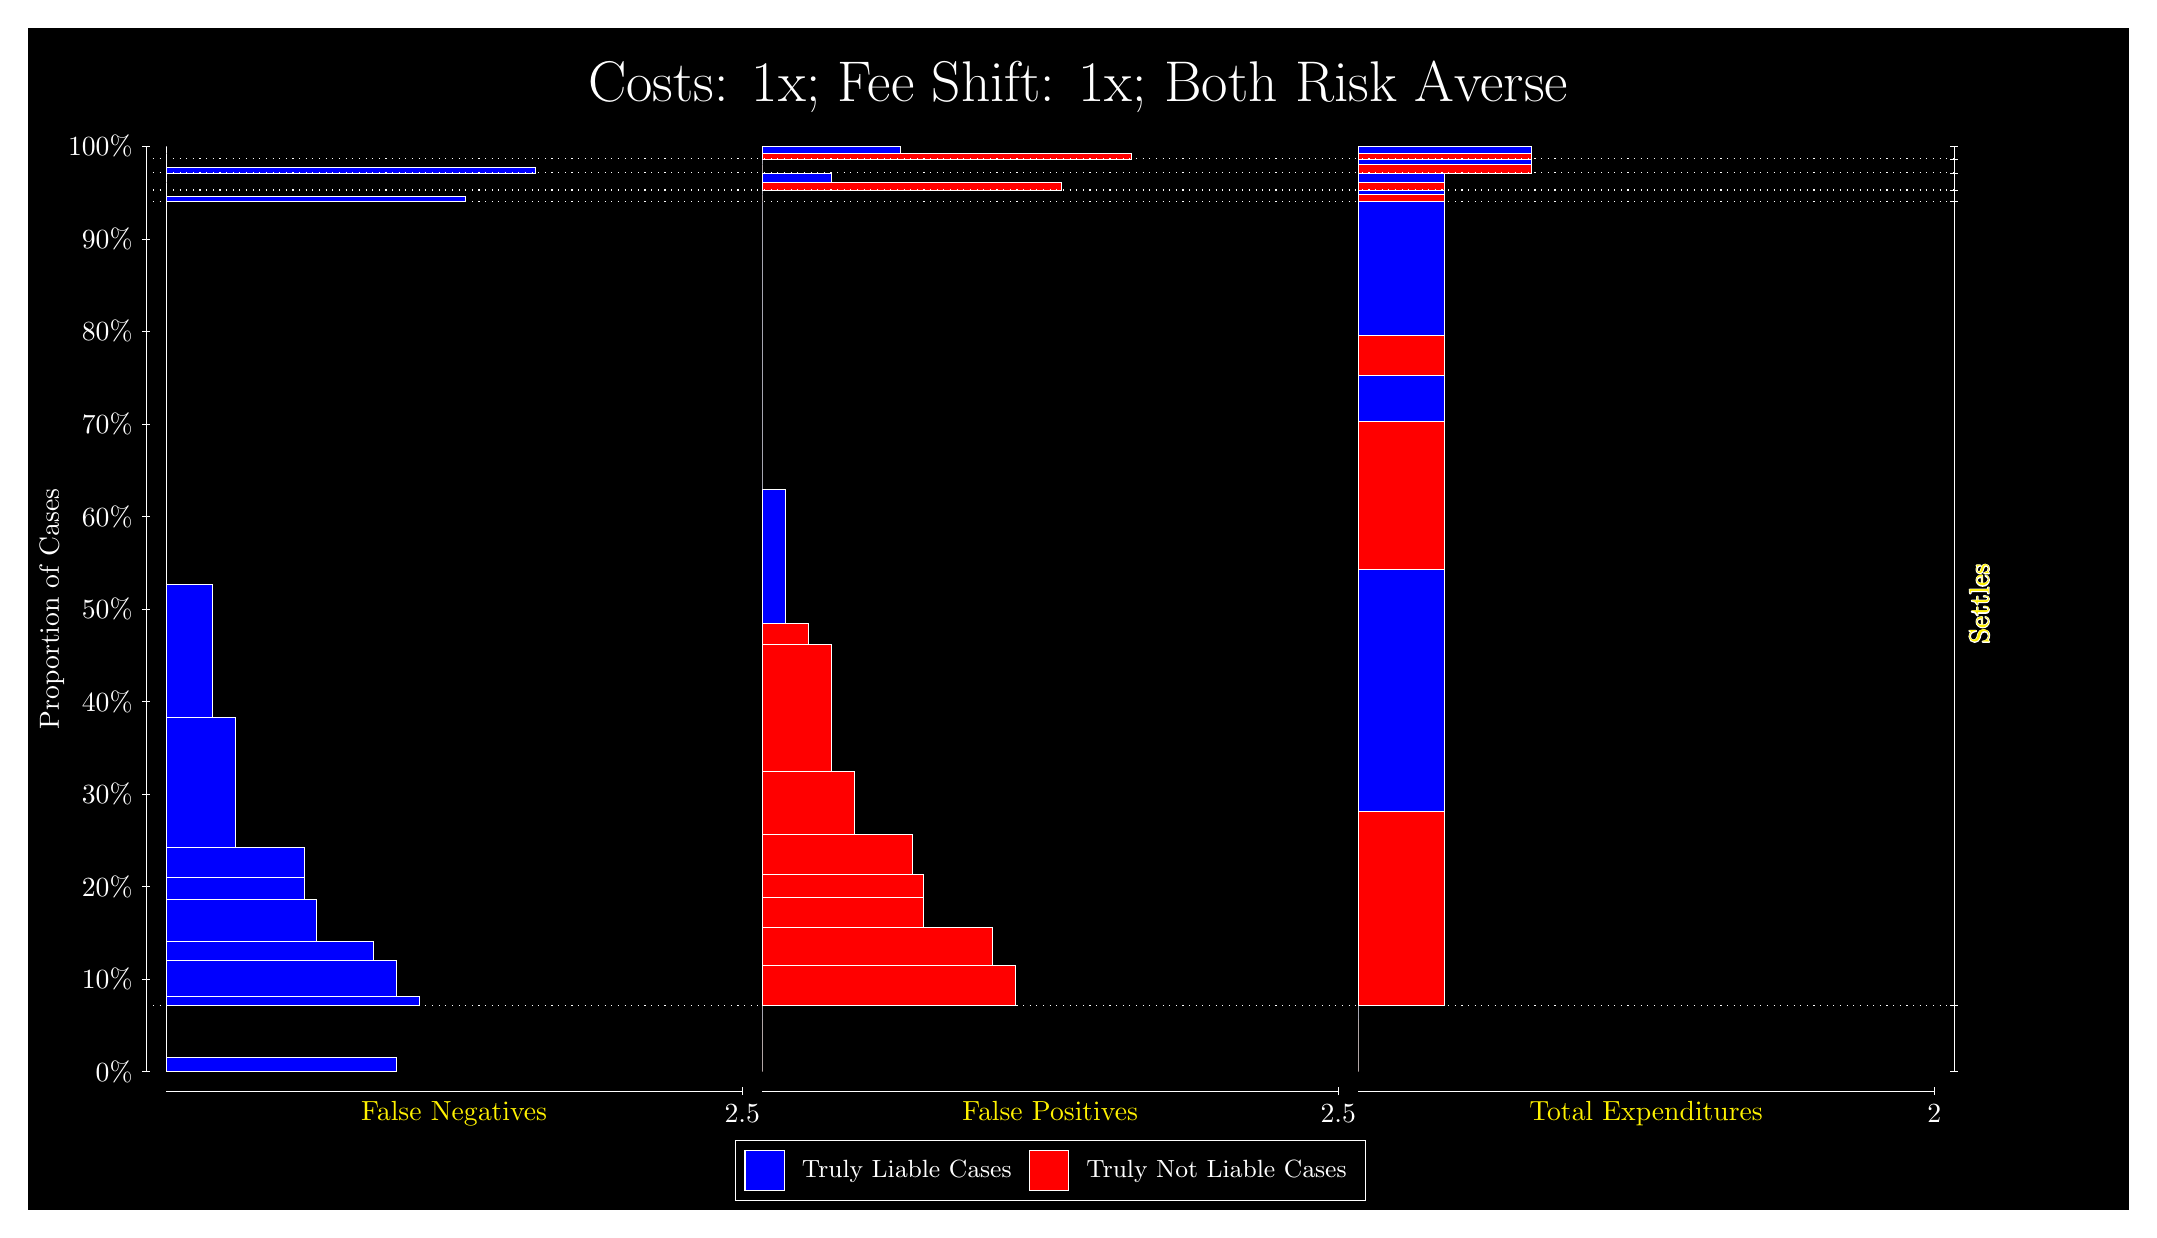
\begin{tikzpicture}
\draw[fill=black] (0,0) rectangle (26.667,15);
\draw[text=white] (0,13.5) rectangle (26.667,15) node[midway] {\huge Costs: 1x; Fee Shift: 1x; Both Risk Averse};
\draw[white, very thin] (1.5,1.75) -- (1.5,13.5);
\node[rotate=90, text=white, anchor=center] at (0.3, 7.625) {Proportion of Cases};
\draw[white, very thin] (1.45,1.75) -- (1.55,1.75);
\node[text=white, anchor=east] at (1.45, 1.75) {0\%};
\draw[white, very thin] (1.45,2.925) -- (1.55,2.925);
\node[text=white, anchor=east] at (1.45, 2.925) {10\%};
\draw[white, very thin] (1.45,4.1) -- (1.55,4.1);
\node[text=white, anchor=east] at (1.45, 4.1) {20\%};
\draw[white, very thin] (1.45,5.275) -- (1.55,5.275);
\node[text=white, anchor=east] at (1.45, 5.275) {30\%};
\draw[white, very thin] (1.45,6.45) -- (1.55,6.45);
\node[text=white, anchor=east] at (1.45, 6.45) {40\%};
\draw[white, very thin] (1.45,7.625) -- (1.55,7.625);
\node[text=white, anchor=east] at (1.45, 7.625) {50\%};
\draw[white, very thin] (1.45,8.8) -- (1.55,8.8);
\node[text=white, anchor=east] at (1.45, 8.8) {60\%};
\draw[white, very thin] (1.45,9.975) -- (1.55,9.975);
\node[text=white, anchor=east] at (1.45, 9.975) {70\%};
\draw[white, very thin] (1.45,11.15) -- (1.55,11.15);
\node[text=white, anchor=east] at (1.45, 11.15) {80\%};
\draw[white, very thin] (1.45,12.325) -- (1.55,12.325);
\node[text=white, anchor=east] at (1.45, 12.325) {90\%};
\draw[white, very thin] (1.45,13.5) -- (1.55,13.5);
\node[text=white, anchor=east] at (1.45, 13.5) {100\%};

\draw[white, very thin] (24.457,1.75) -- (24.457,13.5);
\draw[white, very thin] (24.407,1.75) -- (24.507,1.75);
\node[anchor=west] at (24.407, 1.75) {};
\draw[white, very thin] (24.407,2.5852) -- (24.507,2.5852);
\node[anchor=west] at (24.407, 2.5852) {};
\draw[white, very thin] (24.407,12.8) -- (24.507,12.8);
\node[anchor=west] at (24.407, 12.8) {};
\draw[white, very thin] (24.407,12.945) -- (24.507,12.945);
\node[anchor=west] at (24.407, 12.945) {};
\draw[white, very thin] (24.407,13.164) -- (24.507,13.164);
\node[anchor=west] at (24.407, 13.164) {};
\draw[white, very thin] (24.407,13.341) -- (24.507,13.341);
\node[anchor=west] at (24.407, 13.341) {};
\draw[white, very thin] (24.407,13.5) -- (24.507,13.5);
\node[anchor=west] at (24.407, 13.5) {};

\draw[white, very thin, fill=blue] (1.75,1.75) rectangle (4.6775,1.9291);
\draw[white, very thin, fill=red] (1.75,1.9291) rectangle (1.75,2.5852);
\draw[white, very thin, fill=blue] (1.75,2.5852) rectangle (4.9703,2.7094);
\draw[white, very thin, fill=blue] (1.75,2.7094) rectangle (4.6775,3.168);
\draw[white, very thin, fill=blue] (1.75,3.168) rectangle (4.3848,3.398);
\draw[white, very thin, fill=blue] (1.75,3.398) rectangle (3.6529,3.934);
\draw[white, very thin, fill=blue] (1.75,3.934) rectangle (3.5065,4.2188);
\draw[white, very thin, fill=blue] (1.75,4.2188) rectangle (3.5065,4.5951);
\draw[white, very thin, fill=blue] (1.75,4.5951) rectangle (2.6283,6.2427);
\draw[white, very thin, fill=blue] (1.75,6.2427) rectangle (2.3355,7.9372);
\draw[white, very thin, fill=red] (1.75,7.9372) rectangle (1.75,12.8);
\draw[white, very thin, fill=blue] (1.75,12.8) rectangle (5.5558,12.86);
\draw[white, very thin, fill=red] (1.75,12.86) rectangle (1.75,12.945);
\draw[white, very thin, fill=red] (1.75,12.945) rectangle (1.75,13.042);
\draw[white, very thin, fill=blue] (1.75,13.042) rectangle (1.75,13.164);
\draw[white, very thin, fill=blue] (1.75,13.164) rectangle (6.4341,13.234);
\draw[white, very thin, fill=red] (1.75,13.234) rectangle (1.75,13.341);
\draw[white, very thin, fill=red] (1.75,13.341) rectangle (1.75,13.408);
\draw[white, very thin, fill=blue] (1.75,13.408) rectangle (1.75,13.5);
\draw[white, very thin, fill=red] (9.3189,1.75) rectangle (9.3189,2.4061);
\draw[white, very thin, fill=blue] (9.3189,2.4061) rectangle (9.3189,2.5852);
\draw[white, very thin, fill=red] (9.3189,2.5852) rectangle (12.539,3.0957);
\draw[white, very thin, fill=red] (9.3189,3.0957) rectangle (12.246,3.5818);
\draw[white, very thin, fill=red] (9.3189,3.5818) rectangle (11.368,3.9581);
\draw[white, very thin, fill=red] (9.3189,3.9581) rectangle (11.368,4.2494);
\draw[white, very thin, fill=red] (9.3189,4.2494) rectangle (11.222,4.7633);
\draw[white, very thin, fill=red] (9.3189,4.7633) rectangle (10.49,5.5655);
\draw[white, very thin, fill=red] (9.3189,5.5655) rectangle (10.197,7.1704);
\draw[white, very thin, fill=red] (9.3189,7.1704) rectangle (9.9044,7.448);
\draw[white, very thin, fill=blue] (9.3189,7.448) rectangle (9.6116,9.1425);
\draw[white, very thin, fill=blue] (9.3189,9.1425) rectangle (9.3189,12.8);
\draw[white, very thin, fill=red] (9.3189,12.8) rectangle (9.3189,12.886);
\draw[white, very thin, fill=blue] (9.3189,12.886) rectangle (9.3189,12.945);
\draw[white, very thin, fill=red] (9.3189,12.945) rectangle (13.125,13.042);
\draw[white, very thin, fill=blue] (9.3189,13.042) rectangle (10.197,13.164);
\draw[white, very thin, fill=red] (9.3189,13.164) rectangle (9.3189,13.272);
\draw[white, very thin, fill=blue] (9.3189,13.272) rectangle (9.3189,13.341);
\draw[white, very thin, fill=red] (9.3189,13.341) rectangle (14.003,13.408);
\draw[white, very thin, fill=blue] (9.3189,13.408) rectangle (11.075,13.5);
\draw[white, very thin, fill=red] (16.888,1.75) rectangle (16.888,2.4061);
\draw[white, very thin, fill=blue] (16.888,2.4061) rectangle (16.888,2.5852);
\draw[white, very thin, fill=red] (16.888,2.5852) rectangle (17.986,5.055);
\draw[white, very thin, fill=blue] (16.888,5.055) rectangle (17.986,8.1297);
\draw[white, very thin, fill=red] (16.888,8.1297) rectangle (17.986,10.012);
\draw[white, very thin, fill=blue] (16.888,10.012) rectangle (17.986,10.595);
\draw[white, very thin, fill=red] (16.888,10.595) rectangle (17.986,11.105);
\draw[white, very thin, fill=blue] (16.888,11.105) rectangle (17.986,12.8);
\draw[white, very thin, fill=red] (16.888,12.8) rectangle (17.986,12.886);
\draw[white, very thin, fill=blue] (16.888,12.886) rectangle (17.986,12.945);
\draw[white, very thin, fill=red] (16.888,12.945) rectangle (17.986,13.042);
\draw[white, very thin, fill=blue] (16.888,13.042) rectangle (17.986,13.164);
\draw[white, very thin, fill=red] (16.888,13.164) rectangle (19.083,13.272);
\draw[white, very thin, fill=blue] (16.888,13.272) rectangle (19.083,13.341);
\draw[white, very thin, fill=red] (16.888,13.341) rectangle (19.083,13.408);
\draw[white, very thin, fill=blue] (16.888,13.408) rectangle (19.083,13.5);
\draw[white, dotted] (1.5,2.5852) -- (24.457,2.5852);
\draw[white, dotted] (1.5,12.8) -- (24.457,12.8);
\draw[white, dotted] (1.5,12.945) -- (24.457,12.945);
\draw[white, dotted] (1.5,13.164) -- (24.457,13.164);
\draw[white, dotted] (1.5,13.341) -- (24.457,13.341);
\draw[white, very thin] (1.75,1.5) -- (9.0689,1.5);
\node[text=yellow, anchor=north] at (5.4094, 1.5) {False Negatives};
\draw[white, very thin] (9.0689,1.45) -- (9.0689,1.55);
\node[text=white, anchor=north] at (9.0689, 1.45) {2.5};

\draw[white, very thin] (9.3189,1.5) -- (16.638,1.5);
\node[text=yellow, anchor=north] at (12.978, 1.5) {False Positives};
\draw[white, very thin] (16.638,1.45) -- (16.638,1.55);
\node[text=white, anchor=north] at (16.638, 1.45) {2.5};

\draw[white, very thin] (16.888,1.5) -- (24.207,1.5);
\node[text=yellow, anchor=north] at (20.547, 1.5) {Total Expenditures};
\draw[white, very thin] (24.207,1.45) -- (24.207,1.55);
\node[text=white, anchor=north] at (24.207, 1.45) {2};


\node[text=yellow, centered, rotate=90] at (24.777, 7.6926) {\contour{white}{Settles}};





\draw (12.978300999999998,1.5) node[draw=none] (baseCoordinate) {};
\begin{scope}[align=center]
        \matrix[scale=0.5, draw=white, below=0.5cm of baseCoordinate, nodes={draw}, column sep=0.1cm]{
            \node[rectangle, draw, minimum width=0.5cm, minimum height=0.5cm, fill=blue] {}; &
            \node[draw=none, font=\small, text=white] (B) {Truly Liable Cases}; &
            \node[rectangle, draw, minimum width=0.5cm, minimum height=0.5cm, fill=red] {}; &
            \node[draw=none, font=\small, text=white] (B) {Truly Not Liable Cases}; \\
            };
\end{scope}

\end{tikzpicture}
\end{document}